\section{Durchführung}

\subsection{kleiner 1 bar}
\begin{figure}[H]
    \centering
    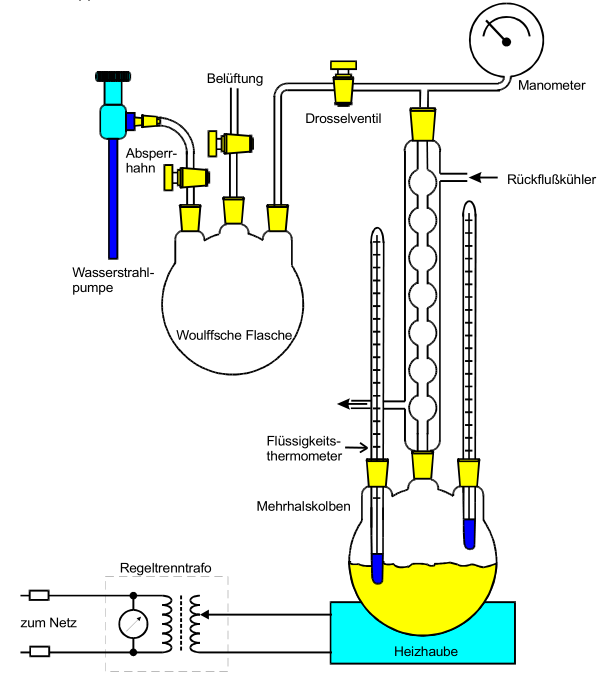
\includegraphics[width=0.55\textwidth]{images/Abbildung3.PNG}
    \caption{Der Versuchsaufbau für Drücke kleiner als 1 Bar.}
    \label{img:aufbau1}
\end{figure}
Für die Messung der Dampfdruckkurve wird die Apperatur aus der Abbildung \ref{img:aufbau1} verwendet. Den realen Aufbau findet man hier \ref{img:real1}  \\
Um ein Vakuum für die Versuchsdurchführung zu erzeugen wird zunächst der Absperrhahn und das Drosselventil geöffnet und das Belülftungsventil geschlossen. 
Die Wasserstrahlpumpe wird nun solange angestellt, bis sich ein konstanter Druck einstellt. 
Dieser Druck ist dabei, unter anderem, abhängig von der Wassertemperatur.\\
Bevor nun die Wasserstrahlpumpe abgeschaltet wird müssen der Absperrhahn und das Drosselventil geschlossen werden. Als nächstes wird nun die Heizhaube 
eingeschalten und gleichzeitig dafür gesorgt, dass Kühlflüssigkeit durch den Rückflusskühler fließt. Falls die Substanz nach ein wenig Zeit 
nicht anfängt zu sieden, kann man noch einmal das Drosselventil öffnen um den Druck innerhalb des Gefäßes weiter zu senken.\\
Anschließend wird bei laufender Heizung regelmäßig die Siedetemperatur und der Dampfdruck abgelesen. Damit höhere Temperaturen erreicht werden können
muss nach einer Weile der Durchfluß der Kühlflüssigkeit reduziert werden, bis die Kühlflüssigkeit nur noch tropft.


\subsection{1 bis 15 bar}
\begin{figure}[H]
    \centering
    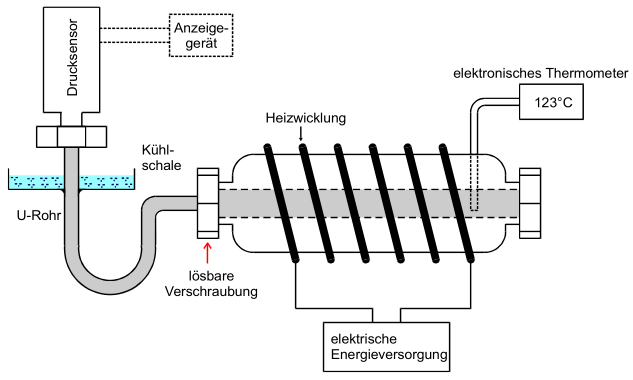
\includegraphics[width=0.55\textwidth]{images/Abbildung4.PNG}
    \caption{Der Versuchsaufbau für den Messbereich von 1 bis 15 Bar.}
    \label{img:aufbau2}
\end{figure}
Die Dampfdruckkurve für Drücke von mehr als einem Bar, wird mit Hilfe  der Apperatur in \ref{img:aufbau2} bestimmt. Ihr reales Äquivalent findet man hier \ref{img:real1}.\\
Um den Versuch zu starten muss zunächst der Hohlraum vollständig mit destilliertem und entgastem Wasser befüllt werden.
Während das Wasser nun langsam erhiztzt wird, liest man die Siedetemperatur und den Sättigungsdampfdruck ab. Dabei ist besonders darauf zu 
achten, dass der Vollauschlag des Manometers nicht überschritten wird. Des Weiteren ist darauf zu auchten, dass das Manometer durch ein mit kaltem Wasser gefülltes 
Kühlbecken vor Erhitzung geschützt.